\subsection{Requirements}
\label{sec:ranked-requirements}

Project requirements define the measurable outcomes of the design process and establish a shared understanding between the client and the development team. Each requirement must be technically sound, verifiable, and achievable within the defined project constraints. 

Requirements were derived from the project brief, client discussions, and technical analysis. Constraints and assumptions were first identified, followed by a prioritisation process based on technical criticality, safety relevance, and feasibility. A detailed record of this process is available in the \textit{Requirements Report}. The ranked requirements are given below in \ref{tab:ranked-req}. The constraints for the requirements can be found in Appendix~\ref{app:constraints}.

\begin{table}[H]
\centering
\caption{Ranked Requirements}
\label{tab:ranked-req}
\begin{tabular}{|>{\centering\arraybackslash}p{0.05\textwidth} | >{\centering\arraybackslash}p{0.07\textwidth} | p{0.65\textwidth} | >{\centering\arraybackslash}p{0.1\textwidth}|}
\hline
\rowcolor{gray!15}
\textbf{Rank} & \textbf{No.} & \textbf{Requirement} & \textbf{Constr.} \\
\hline
1 & R.2  & The drone shall be capable of hovering and flying. & C.1 \\
\hline
2 & R.30 & The drone must power off after 30~s of disconnection. & C.6 \\
\hline
3 & R.1  & The drone shall operate in an indoor area. & C.3 \\
\hline
4 & R.17 & The drone shall utilise shrouded propellers or propeller guards. & C.6 \\
\hline
5 & R.3  & The drone shall navigate without the use of \gls{gps}. & C.3 \\
\hline
6 & R.4  & The drone shall maintain a set hovering altitude during autonomous
surveillance. & C.3 \\
\hline
7 & R.14 & A manual override system shall be available to the user. & C.2, C.7 \\
\hline
8 & R.27 & The drone shall autonomously land safely when battery levels are low. & C.
3 \\
\hline
9 & R.24 & Any third-party software used for control must be open-source and freely available. & C.2 \\
\hline
10 & R.23 & The drone design shall remain within a budget of \textdollar350.00. & C.4 \\
\hline
11 & R.20 & The drone shall be capable of flight stabilisation. & C.2, C.7 \\
\hline
12 & R.5  & The drone shall maintain a default altitude between 1.2--1.3m during operation. & C.2 \\
\hline
13 & R.18 & Power shall be supplied by one 1S or 2S \gls{lipo} battery (<800~mAh). & C.6 \\
\hline
14 & R.15 & The flight controller shall use a custom PCB integrating sensors and power distribution. & C.2 \\
\hline
15 & R.21 & The drone shall maintain stability under wind disturbances. & C.2, C.7 \\
\hline
\end{tabular}
\end{table}

The system must operate reliably in confined indoor environments, maintain stable and controllable flight without GPS, and integrate safety mechanisms that protect both users and equipment. Core requirements prioritise flight stability, communication reliability, and compliance with weight, power, and cost limits. Lower-priority requirements cover enhancements such as diagnostics, video capability, and improved user interface feedback.

There are also several lower-priority requirements that are not essential to meeting the primary project goals but remain background considerations. These features may still be implemented if they can be added with minimal time or resource overhead. The additional requirements are given in Appendix~\ref{app:additional_req}.

The ranked requirements form the foundation for architectural, hardware, and software decisions presented in the following sections.

%----------------------------------------------------------------%
\subsection{Design Architecture}

The design architecture defines how major subsystems interact to meet functional, safety, and performance requirements. It establishes clear boundaries between sensing, control, communication, and actuation components, ensuring reliable operation and outlining the integration of these components with each other.

While the desired behaviour of the system establishes its requirements, along with additional factors such as safety considerations and other constraints that influence the final design, the system architecture represents the high-level realisation of these requirements. It defines the main function elements of the system and the interfaces between them. Based on this architecture, specific design components are then selected to best implement the intended functionality.

\begin{figure}[H]
    \centering
    \captionsetup{justification=centering, margin=1cm}
    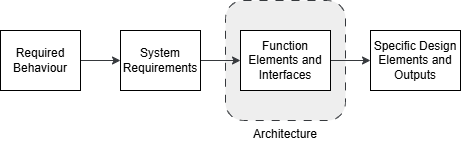
\includegraphics[width=0.65\textwidth]{img/arch-process.PNG}
    \caption{System Architecture Process}
    \label{fig:arch-process}
\end{figure}

%-------------------------------------------------------------%
\subsubsection{Overall Architecture}

The overall system architecture, shown in Fig.~\ref{fig:block-overall}, is divided into three main layers: the User–Web Interface, the Web–Firmware Interface, and the Firmware–Hardware Interface. These layers communicate through well-defined protocols to ensure reliable and modular operation.

\begin{figure}[H]
    \centering
    \captionsetup{justification=centering, margin=1cm}
    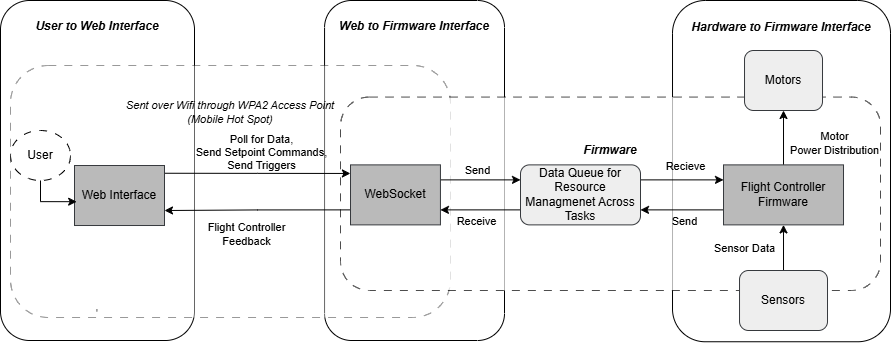
\includegraphics[width=0.95\textwidth]{img/block-overall-gray.PNG}
    \caption{Overall System Architecture with Hardware and Firmware Interfaces}
    \label{fig:block-overall}
\end{figure}

\textbf{User to Web Interface}: The operator controls the drone and monitors system feedback via a web interface supporting both manual and autonomous flight. Real-time telemetry, sensor feedback, and emergency motor shutdown are provided over a WPA2-secured Wi-Fi connection.

\textbf{Web to Firmware Interface}: A persistent WebSocket link connects the web interface and the flight controller. Three message types are supported: (i) \textit{data requests} for sensor feedback, (ii) \textit{setpoint commands} for control updates, and (iii) \textit{control triggers} for testing or initiating sequences. The WebSocket and control processes run as independent \gls{rtos} tasks, communicating via thread-safe queues to prevent race conditions.

\textbf{Firmware to Hardware Interface}: The flight controller directly interfaces with onboard sensors and motor drivers. Sensor data is continuously processed to generate thrust commands that maintain stable flight. The control loop responds in real time to user or autonomous inputs, ensuring stable hover and smooth manoeuvres.

The design philosophy for the indoor \gls{uav} is founded on the principles of simplicity, modularity, and maintainability, ensuring a system that is functional, safe, and adaptable within its operating environment. Simplicity reduces unnecessary complexity and potential failure points, modularity enables independent development and integration of subsystems, and maintainability supports long-term reliability through ease of repair and clear documentation. These principles are reinforced by high-level design considerations - functionality, safety, cost-effectiveness, sustainability, reliability, and usability - ensuring that the final system achieves stable, efficient, and safe autonomous flight in confined indoor environments.

The following sections describe the hardware and firmware architectures in further detail.

%-------------------------------------------------------------%
\subsubsection{Hardware Architecture}

The hardware architecture integrates sensing, control, communication, and power management into a single lightweight \gls{pcb} mounted on a 3D printed frame. Fig.~\ref{fig:block-hardware} illustrates the main components and their interconnections. 

\begin{figure}[H]
    \centering
    \captionsetup{justification=centering, margin=1cm}
    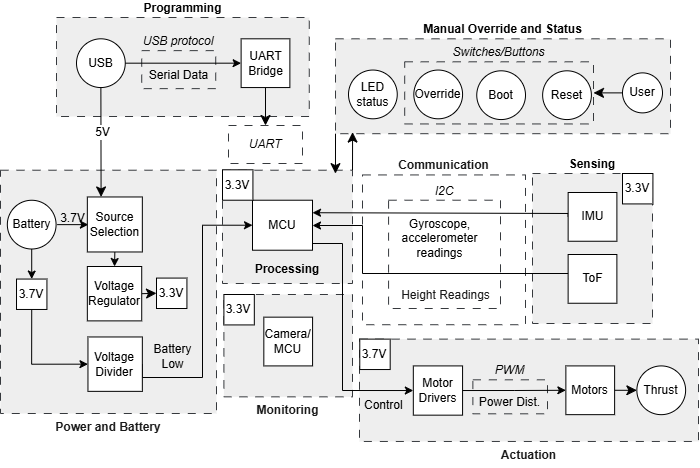
\includegraphics[width=0.8\textwidth]{img/block-hardware-gray.PNG}
    \caption{Hardware Architecture}
    \label{fig:block-hardware}
\end{figure}

A description of each of the architectural elements is given below in Table~\ref{tab:hardware-arch}.  ach element of the hardware architecture supports a specific functional or safety requirement, as outlined in Table~\ref{tab:hardware-arch}. Additionally, the \gls{pcb} design must maintain signal integrity, minimise power losses, and allow efficient component routing (R.15). The structural frame supports the \gls{pcb}, battery, and motors, incorporating propeller guards to satisfy safety requirements (R.17).

\begin{table}[H]
\centering
\caption{Hardware Elements and Requirements}
\label{tab:hardware-arch}
\begin{tabular}{|m{0.25\textwidth}|m{0.50\textwidth}|m{0.20\textwidth}|}
\hline
\rowcolor{gray!15}
\textbf{Architectural Element} & \textbf{Purpose} & \textbf{Requirement(s)} \\
\hline
Actuation and Sensing & Provides continuous data needed for state estimation (position and orientation of the drone), control stability, and safety. & R.2, R.1, R.3, R.4, R.20, R.5, R.21 \\
\hline
Power and Battery  & Regulates power supply input and manages power from battery. & R.27, R.18 \\
\hline
Processing, Programming, Communication & \gls{mcu} executes control loops and manages peripheral communication. \newline
Programming allows firmware upload and monitoring of diagnostics. \newline
Communication provides telemetry between sensors, actuators, and processing tasks. & All except R.17, R.14, R.18, R.15 \\
\hline
Actuation & Converts control signals into thrust outputs. & R.2, R.1, R.4, R.27, R.29, R.5 \\
\hline
Manual Override and Status & Provides manual override and status via LEDs. & Additional \\
\hline
Monitoring & Provides a means for surveillance of the environment. & Additional \\
\hline
\end{tabular}
\end{table}

%-------------------------------------------------------------%
\subsubsection{Hardware Justification}

The architecture was informed by several open-source designs, including CircuitDigest’s ESPDrone \cite{espdrone_circuitdigest}, Espressif’s ESP-Drone \cite{espdrone_espressif}, and Max Imagination’s ESP-FLY \cite{maximagination}, alongside Espressif’s official ESP32 DevKit schematics \cite{espressif_devkits}. These references provided practical guidance for lightweight drone design, component selection, and standard circuit integration. The final design integrates these layouts with project-specific adaptations to meet the functional and safety requirements of this project. The design elements and the rationale behind them is given in Table~\ref{tab:hardware-justification}.

\renewcommand{\arraystretch}{1.2}
\begin{table}[H]
\centering
\caption{Design Element Justification}
\label{tab:hardware-justification}
\begin{tabular}{|p{0.18\textwidth}|p{0.82\textwidth}|}
\hline
\rowcolor{gray!15}
\textbf{Element} & \textbf{Rationale} \\
\hline
Power and Battery & The ESP32 requires a stable 3.3\,V supply. A source selection circuit allows both battery and \gls{usb} connection, with priority given to \gls{usb}. Battery low level is monitored via simple voltage divider to warn when charge is low. \\
\hline
Programming & Firmware uploading and debugging require a \gls{usb}-to-\gls{uart} bridge, providing direct serial communication with the \gls{mcu}. \\
\hline
Sensing and Communication & An \gls{imu} is necessary for flight stability and position control. A \gls{tof} sensor simplifies height measurement and reduces error accumulation from integration. Sensors use standard protocols such as I\textsuperscript{2}C for reliable communication with the \gls{mcu}. \\
\hline
Actuation & \gls{dc} motors controlled via \gls{pwm} generate thrust. Individual motor control ensures balance and stabilisation. Simple motor driver circuits (\glspl{ic} or \gls{mosfet} switches) provide reliable control for each motor. \\
\hline
Monitoring & A separate \gls{mcu} for the surveillance camera ensures independent processing from the flight controller for modularity. \\
\hline
Manual Override and Status & Physical switches and LEDs provide user feedback and safety. Manual power-off allows immediate shutdown. Status LEDs indicate power and connectivity. \\
\hline
\end{tabular}
\end{table}

%----------------------------------------------------------------%
\subsubsection{Firmware Architecture}
The firmware architecture defines the drone’s control logic and operational behaviour. It manages sensor acquisition, state estimation, and motor actuation within a real-time stabilisation loop. Sensor fusion combines \gls{imu} and time-of-flight (\gls{tof}) data to estimate orientation and altitude, while cascaded \gls{pid} controllers maintain attitude and height stability.  

A WebSocket-based communication layer enables remote telemetry and command control via a Wi-Fi access point. Safety routines include manual override and automatic motor shutdown in case of communication loss or detected fault conditions.

\begin{figure}[H]
    \centering
    \captionsetup{justification=centering, margin=1cm}
    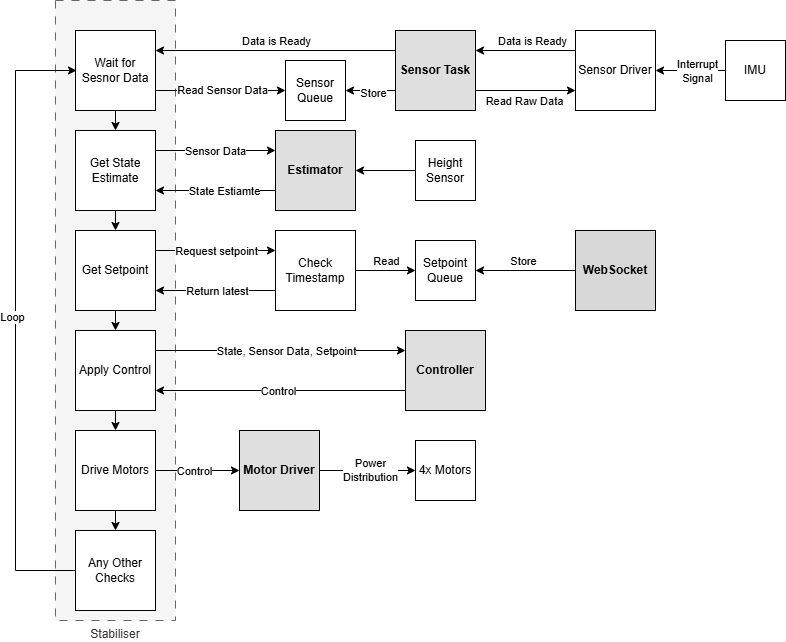
\includegraphics[width=0.98\textwidth]{img/block-software-gray2.PNG}
    \caption{Firmware Architecture}
    \label{fig:block-software}
\end{figure}

%----------------------------------------------------------------%
\subsubsection{Firmware Justification}

Firmware using the ESP32 was reviewed for the firmware architecture including Espressif’s ESP-Drone (or more so, Circuit Digest’s modified version~\cite{espdrone_circuitdigest}, with fixed UDP driver needed for Crazyflie Client (CFClient)). It is built on the \gls{esp-idf} framework and derived from the Crazyflie open-source project (GPL-3.0)~\cite{bitcraze_crazyflie_firmware} and was assessed as a baseline for stable flight and mobile control. Phadte’s ESP32 Flight Controller~\cite{pratikphadte_flight_controller} developed with the Arduino framework, was reviewed as a simple custom implementation of a flight controller, built for a larger brushless motor drone, and the \gls{pid} tuning methodology.  

Based on this analysis, a custom firmware was developed using \gls{esp-idf} v5.5.0 to provide long-term flexibility, low-level control, and improved integration. This approach simplified the generalised Crazyflie libraries of ESP-Drone, which contain dozens of source files and many macros and generalisations to work with multiple drone designs. Then, the lower-level \gls{esp-idf} environment was chosen over Arduino to achieve more precise timing, and compatibility with \gls{esp-idf} libraries.

This configuration ensures stable flight under constrained indoor conditions while maintaining extensibility for future autonomous functionality and research development within the \gls{uwaal}.

\begin{table}[H]
\centering
\renewcommand{\arraystretch}{1.2}
\caption{Firmware Option Comparison}
\begin{tabular}{|>{\bfseries}p{0.17\textwidth}|p{0.2\textwidth}|p{0.2\textwidth}|p{0.2\textwidth}|}
\hline
\rowcolor{gray!15}
\textbf{Feature} & \textbf{ESP-Drone} & \textbf{Phadte} & \textbf{Custom} \\
\hline
Framework & \gls{esp-idf} v4.4.8 & Arduino & \gls{esp-idf} v5.5.0 \\
\hline
Control Type & Manual & Manual & Manual/Autonomous \\
\hline
Complexity & High & Low & Moderate \\
\hline
Flexibility & Moderate & Low & High \\
\hline
Integration & \gls{esp-idf} libraries & Arduino libraries & \gls{esp-idf} libraries \\
\hline
Primary Focus & General purpose & Flight stabilisation only & Project specific \\
\hline
\end{tabular}
\end{table}

The final architecture balances flexibility and control, centring on a stabilisation loop that integrates \gls{imu} feedback, cascaded \gls{pid} control, and motor actuation derived from the Crazyflie core library, as shown in Fig.~\ref{fig:block-software}.

\begin{table}[H]
\centering
\caption{Firmware Architecture Rationale}
\renewcommand{\arraystretch}{1.2}
\begin{tabular}{|p{0.16\textwidth}|p{0.25\textwidth}|p{0.49\textwidth}|}
\hline
\rowcolor{gray!15}
\textbf{Element} & \textbf{Purpose} & \textbf{Rationale} \\
\hline
Sensor Task & Acquire data from onboard sensors. & Sensor inputs are required to estimate the drone’s state. \gls{imu} and \gls{tof} sensors were used to meet project requirements while remaining compatible with open-source third-party software if needed. \\
\hline
State Estimator & Combine sensor inputs to estimate attitude (roll, pitch, yaw) and altitude. & State estimation is necessary for the drone to determine its orientation, needed for stabilisation. \\
\hline
Motor Driver & Convert control signals into motor speed commands via \gls{pwm} or driver interface. & Motor control generates thrust based on output from the \gls{pid} control system. \\
\hline
Override & Handle manual override, loss of communication, and fault detection. & Safety functions include fault detection, manual override, and controlled handling of errors to prevent unsafe operation. \\
\hline
Communication & Provide telemetry, control input, and data logging through WebSocket or serial link. & Communication with the WebSocket is required for remote activation or deactivation, command transmission, and system feedback. It also supports debugging and monitoring. \\
\hline
Timing/Stabiliser & Coordinate execution timing using an \gls{rtos}. & Timing management is critical for stabilisation, ensuring rapid response to changes in drone position or environment. \\
\hline
User Interface & Present data and system status to the operator via wireless connection. & The user interface enables remote deactivation, monitoring of system status, and basic control of the drone. \\
\hline
\end{tabular}
\end{table}